\section{Análisis}

En esta sección presentaremos el análisis de los distintos casos de estudio abordados. Cada subsección corresponderá a uno de ellos, abordándolos de menor a mayor tamaño.

\subsection{Red doméstica}

\subsection{Nodos intervinientes}
\textcolor{red}{HACER ESTE GRAFICO CON LA CASA DE MAXI!}
\begin{figure}[h!]
    \centering                                                       
    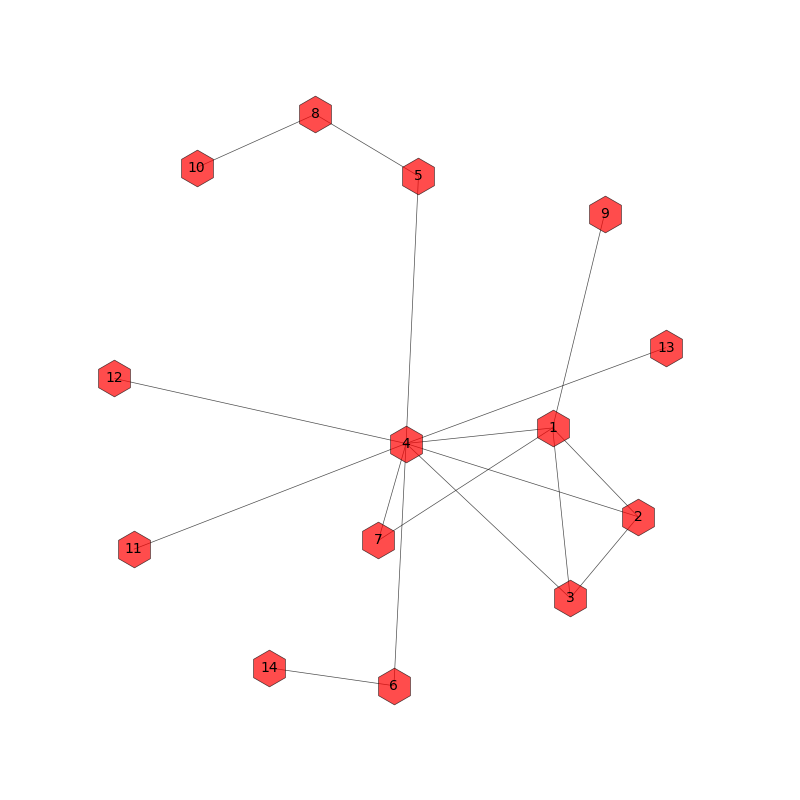
\includegraphics[width=300pt]{img/laboralGraph.png}
    \caption{Grafo de Red Laboral}
    \label{laboral:graph}
\end{figure}

\subsection{Frecuencia de los distintos tipos de paquetes}

% En el gráfico \ref{domestica:paquetes} se pueden ver los resultados de obtenidos.

% \begin{figure}[h!]
%     \centering                                                       
%     \includegraphics[width=300pt]{img/"Red Doméstica - Frecuencias en función de tipos de paquetes.png"}
%     \caption{}
%     \label{domestica:paquetes}
% \end{figure}

\subsection{Información de las fuentes emisoras y receptoras de paquetes ARP.}

Para realizar este caso comparamos la información proporcionada por las fuentes emisoras de paquetes ARP e ilustramos asimismo la entropía de la fuente. Los resultados se pueden observar en los gráficos \ref{domestica:emisoras} y \ref{domestica:receptoras}

\begin{figure}[h!]
    \centering                                                       
    \includegraphics[width=300pt]{img/"Red Doméstica - Información de las fuentes emisoras de paquetes ARP.png"}
    \caption{}
    \label{domestica:emisoras}
\end{figure}

En el primero de ellos se ve que existe una única fuente situada por debajo de la entropía y corresponde a la IP 169.254.93.30. La baja información que aporta indica que se trata de un nodo que emite muchos paquetes ARP. En contraposición, las IP 192.168.0.103 y 192.168.0.100 muestran un gran aporte de información, de lo cual se deduce que es poco común que las mismas envíen paquetes de solicitud ARP.


\begin{figure}[h!]
    \centering                                                       
    \includegraphics[width=300pt]{img/"Red Doméstica - Información de las fuentes receptoras de paquetes ARP.png"}
    \caption{}
    \label{domestica:receptoras}
\end{figure}

En el segundo gráfico se observa una entropía mayor. De esto podría deducirse que es una fuente aún más aleatoria y menos predecible que la que filtra únicamente los envíos de paquetes ARP.\\
En este caso, los nodos distinguidos son - por su gran valor de información - los que mapean las direcciones IP 192.168.0.103, 192.168.0.9 y 192.168.0.111 y, por su poca cantidad de información el nodo 0.0.0.0, seguido del 169.254.93.30. Esto indica que frecuentemente se realizan requests a estos últimos hosts, mientras que los primeros son ignorados la mayor parte del tiempo. \\
\textcolor{red}{ver si tiene alguna relacion con la forma en q estan dispuestos en el grafo!}

¿Por qué es tan frecuente que se realicen solicitudes al host cuya IP es 0.0.0.0? Podríamos pensar que se trata de comunicaciones que un nodo envía a sí mismo pero también cabría suponer - de acuerdo a lo investigado - que puede tratarse de un mecanismo de chequeo de IP's duplicadas en la red.\\

Comparando ambos gráficos podríamos decir que es bastante común que la IP 169.254.93.30 envíe y reciba paquetes ARP. Es por eso que consideramos que podría ser un potencial candidato a Router. \textcolor{red}{verificar con el grafo.}

\newpage
\subsection{Red Laboral}

En este segundo caso, se analizó una red laboral de una PyME. La captura se realizó por un lapso de media hora en modo promiscuo.

\subsection{Nodos intervinientes}
En el gráfico \ref{laboral:graph} se pueden ver los resultados de obtenidos.

\begin{figure}[h!]
    \centering                                                       
    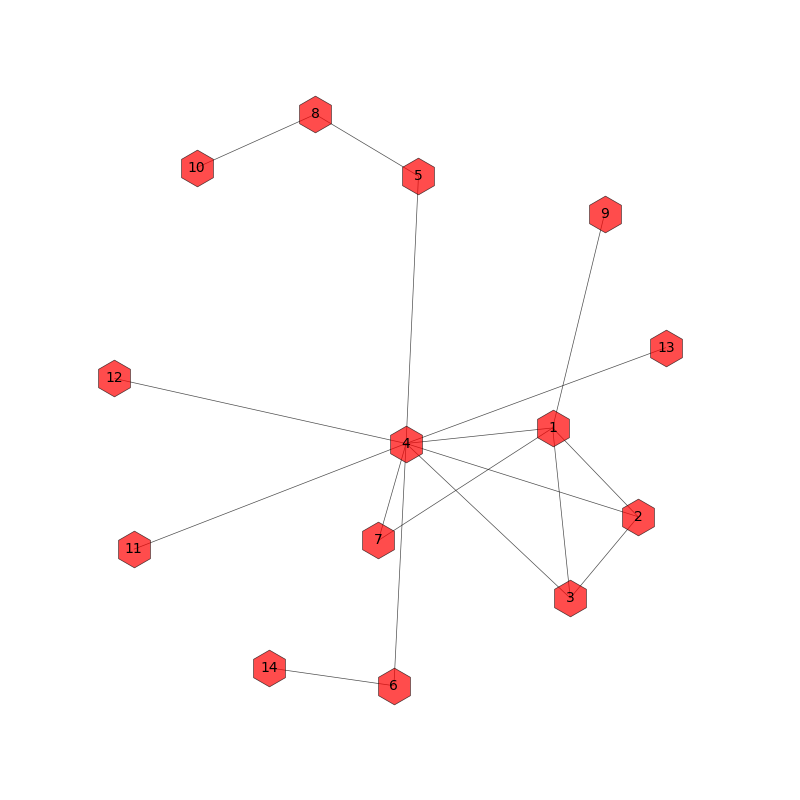
\includegraphics[width=300pt]{img/laboralGraph.png}
    \caption{Grafo de Red Laboral}
    \label{laboral:graph}
\end{figure}

La visualización del grafo indicaría, a primera vista, que el nodo 4 se transmite paquetes con la mayoría de los demás vértices (excepto casos particulares) siendo el candidato ideal para ser el router de esta conexión - es decir, el nodo con salida exterior.\\

El nodo 1 también se comunica con varios nodos a la vez - esto se debe a que es un servidor local en la oficina, al cual le llegan peticiones de nodos particulares - que a su vez también se comunican con los otros que acceden a dicho servidor local. Es decir, el nodo 2, 3, 7 y 9 acceden al servidor local 4, pero a su vez entre el 2 y el 3 se comunican entre ellos.\\

Los nodos 10, 8 y 14 parecieran ser nodos particulares que no se conectan con el router. En particular, el nodo 8 es 0.0.0.0, por lo que en realidad es el nodo 5 y 10 comunicándose con ellos mismos . El nodo 14 es una IP interna así que posiblemente es un nodo comunicándose con una interfaz propia.\\

Luego de ese análisis, consultamos las IPs con la configuración de la red (a la que tenemos acceso por ser la red de la oficina laboral). Efectivamente, el nodo 4 es el router, así como el nodo 1 el servidor local estimado, y los nodos 2, 3, 7 y 9 los que se comunican con dicho servidor.

La incertidumbre del nodo 14 se resolvió como una Virtual Network Adapter, producto de una Virtual Box corriendo en el nodo 6.

Todas las demás relaciones parecen ser naturales, de nodos que se comunican con el router para poder salir a internet.

\subsection{Frecuencia de los distintos tipos de paquetes}

En el gráfico \ref{laboral:paquetes} se pueden ver los resultados de obtenidos. Allí se observa la predominancia de los paquetes de tipo IPV4. Esto tiene sentido, puesto que en este contexto es más frecuente el intercambio de paquetes a nivel de Internet que el realiazado a nivel de la intranet, con la cual las computadoras se encuentran conectadas a través de Ethernet \textcolor{red}{ESTO ES ASI? CORREGIR SI NO POR FAVOR}.

\begin{figure}[h!]
    \centering                                                       
    \includegraphics[width=300pt]{img/"Red Laboral - Frecuencia en función de tipos de paquetes.png"}
    \caption{}
    \label{laboral:paquetes}
\end{figure}

Comparando las figuras \ref{laboral:emisoras} y \ref{laboral:receptoras} se puede ver que las fuentes receptoras superan en cantidad a las fuentes emisoras.\\

\subsection{Información de las fuentes emisoras y receptoras de paquetes ARP.}

\begin{figure}[h!]
    \centering                                                       
    \includegraphics[width=300pt]{img/"Red Laboral - Información de las fuentes emisoras de paquetes ARP.png"}
    \caption{}
    \label{laboral:emisoras}
\end{figure}

Dentro de las IPs emisoras se puede destacar la participación activa de el nodo 192.168.1.1, la cuál aporta un valor muy pequeño de información, encontrándose por debajo de la entropía. Esto indicaría que se trata del host que más paquetes ARP envía dentro de la red. \\

\begin{figure}[h!]
    \centering                                                       
    \includegraphics[width=300pt]{img/Red Laboral - Información de las fuentes receptoras de paquetes ARP.png}
    \caption{}
    \label{laboral:receptoras}
\end{figure}

Si lo buscamos en el gráfico \ref{laboral:receptoras}, el mismo nodo aporta una información por encima de la media, pero sin ser destacada. Esto puede deberse a que se trata del Router, el cual debe encargarse de hacer llegar a todo vértice de la red que coordina los mensajes que se transmiten a través de él.\\
Otro caso a destacar es el de la IP 192.168.1.157 (nodo 7). Este nodo se encuentra en la figura \ref{laboral:receptoras} como aquel que menos información reporta, es decir, como el que más frecuentemente recibe requests. \\ \textcolor{red}{POR QUE SERA ASI SI NO ES NI SERVER NI ROUTER? NO SE COMO EXPLICARLO}


\newpage
\subsection{Red Bonafide}
 Por último, dadas las peque\~nas dimensiones de las redes anteriores, decidimos tomar datos de la red pública ofrecida por el local Bonafide. La captura se realizó por un lapso de media hora en modo promiscuo.

\subsection{Nodos intervinientes}

En el gráfico \ref{bonafide:graph} se pueden ver los resultados de obtenidos.

\begin{figure}[h!]
    \centering                                                       
    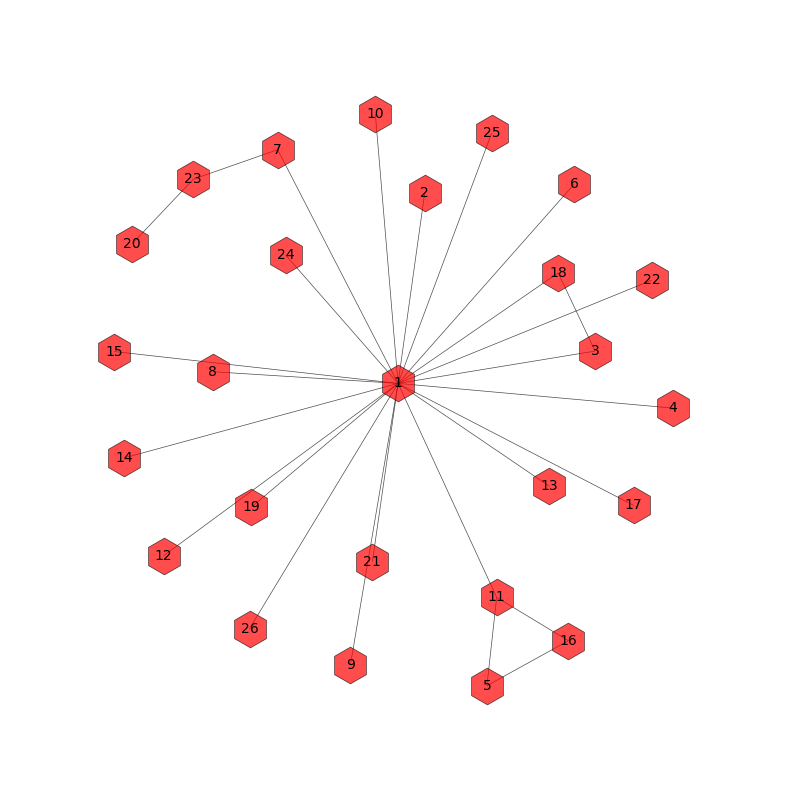
\includegraphics[width=300pt]{img/bonafideGraph.png}
    \caption{Grafo de Red Bonafide}
    \label{bonafide:graph}
\end{figure}
Si bien el grafo resultante no es exactamente la idea previa que teníamos de él (un grafo estrella con el nodo root como raíz) resulta interesante observar la indiscutible predominancia de aristas incidentes al nodo 1, descripto con la dirección IP 192.168.1.1: el resto de los nodos son adyacentes a él o tienen un camino al mismo de - a lo sumo - tercer grado.\\
Consideramos que estos datos son suficientes como para deducir que dicha dirección IP coincide con la del router.\\
Al indagar acerca de la naturaleza de los únicos nodos que no se encuentran conectados de forma directa al nodo 1 (el 5 (192.168.1.110), el 16 (192.168.1.4), el 23(0.0.0.0) y el 20 (169.254.201.232)) llegamos a las siguientes conclusiones: \\
\begin{itemize}
	\item Tanto el nodo 5 como el 16 (ambos de clase C) se comunican con el router a través del nodo 11 (192.168.1.105). Ahondando en las características de estas transferencias, se puede ver que el nodo 11 realiza requests a los nodos 1, 5 y 16, pero sólo llega a él un request desde el nodo 16. Podríamos entonces inferir que el nodo 11 puede estar funcionando como switch \textcolor{red}{FRUTA FRUTA FRUTA PARA TODOS. AVERIGUAR ESTO Y CORREGIRLO.}
	\item El nodo 20 se conecta al 23 y éste último al 7 (192.168.1.100). Esto forma la secuencia 169.254.201.232 (clase B)- 0.0.0.0 - 192.168.1.100 (clase C) - router. Si bien no se trata de un grafo dirigido, se puede ver en los resultados que la dirección 0.0.0.0 nunca recibe datos que podamos escuchar, si no que envía requests a ambos nodos que lo circundan.\\ De acuerdo a lo investigado, inferimos que se trata de un fenómeno que ocurre cuando un nuevo host se conecta a la IP, con el fin de verificar que no tenga una dirección que se encuentre en uso, evitando así las IP duplicadas.\\
\end{itemize}


\subsection{Frecuencia de los distintos tipos de paquetes}

En el gráfico \ref{bonafide:paquetes} se pueden ver los resultados de obtenidos.

\begin{figure}[h!]
    \centering                                                       
    \includegraphics[width=300pt]{img/"Red Bonafide - Frecuencias en función de tipos de paquetes.png"}
    \caption{}
    \label{bonafide:paquetes}
\end{figure}

\subsection{Información de las fuentes emisoras y receptoras de paquetes ARP.}

\begin{figure}[h!]
    \centering                                                       
    \includegraphics[width=300pt]{img/"Red Bonafide - Información de las fuentes emisoras de paquetes ARP.png"}
    \caption{}
    \label{bonafide:emisoras}
\end{figure}

\begin{figure}[h!]
    \centering                                                       
    \includegraphics[width=300pt]{img/"Red Bonafide - Información de las fuentes receptoras de paquetes ARP.png"}
    \caption{}
    \label{bonafide:receptoras}
\end{figure}




% \indent Vamos a comenzar mencionando ciertas particularidades que notamos al mirar un poco los datos:
% \begin{itemize}
% 	\item Por los números de las direcciones IP, se trata de una red clase A (dentro del rango 0.0.0.0 a 127.255.255.255).
% 	\item A diferencia de lo usual, los que suponemos, son routers, tienen direcciones que terminan distinto a ``.1'' (por ejemplo: ``.254'' o ``.230''). Eso es configurable por el administrador de red, y según pudimos averiguar, aparte de estilarse tener los \textit{gateway} finalizando en ``.1'', también se suele guardar las primeras direcciones para nodos particulares como servidores o impresoras, dejando las últimas direcciones para gateways, como inferimos que sucede en este caso.
% \end{itemize}
% \indent Para no repetir el análisis granular similar al punto anterior, vamos a trabajar con la muestra grande, que se corresponde con todos los paquetes capturados.

% \indent Las entropías calculadas para ambas fuentes son:\\

% \begin{center}
% 	\begin{tabular}{ | c | c | c |} \hline
% 	   & \textbf{$S_{src}$} & \textbf{$S_{dst}$} \\ \hline
% 	  	\textbf{Entropía} & 6,29 bits & 5,40 bits \\ \hline
% 	\end{tabular}
% \end{center}

% \indent Como en los análisis anteriores, se realizaron gráficos de barras con la información contenida en los símbolos de las fuente con una recta que representa la entropía de la fuente para contrastar. Recordamos que solamente mostramos en los gráficos los símbolos con menor información, es decir aquellos que son suficientes para realizar el análisis pertinente.\\

% \indent Para la fuente \textit{Fuente}, se obtuvo el siguiente gráfico:\\

% \begin{center}
% \includegraphics[scale=0.5,clip=true,trim=100 0 0 0]{graphics/facultad_grande_src.png}
% \end{center}

% \indent En contraste con los casos de estudio anteriores, parecería que aquí una mayor cantidad de nodos cumplen con el criterio que establecimos para ser considerados como nodos distinguidos. El que menos información contiene es la IP 10.2.100.254.\\

% \indent Para la fuente destino:\\
% \begin{center}
% \includegraphics[scale=0.5,clip=true,trim=100 0 0 0]{graphics/facultad_grande_dst.png}
% \end{center}
% \indent Se pueden observar claramente cuatro IPs que podríamos considerar distinguidas y una, la 169.254.255.255 con un valor muy similar a la entropía de la fuente.\\

% \indent Concentrándonos en estos candidatos de nodos distinguidos, analizamos el grafo dirigido que representa la captura con el fin de determinar si los resultados se verifican gráficamente como nodos relevantes. Logramos ver que efectivamente hay una relación, y los nodos que sobresalen en los gráficos. son los que más flechas tienen (desde o hacia ellos, según corresponda) en los grafos.\\
% \\
% \indent Esta sería toda la red:\\
% \begin{center}
% \includegraphics[scale=0.5,clip=true,trim=140 0 0 0]{graphics/toda_la_red.png}
% \end{center}
% \newpage
% \indent Por supuesto, este gráfico no parece indicarnos nada a esta escala.\\
% \indent Si nos acercamos a algunos de los que catalogamos distinguidos, como el nodo 0.0.0.0 del que salen muchos pedidos y no llega ninguno (en sintonía con el análisis realizado que determinaba que era un nodo distinguido para la fuente origen), y el que suponemos es un router (10.2.100.254) del que salen y llegan muchos pedidos, justificando su aparición como nodo distinguido en ambas fuentes:\\

% \begin{center}
% \includegraphics[scale=0.5,clip=true,trim=140 0 0 0]{graphics/distinguidos.png}

% \includegraphics[scale=0.3,clip=true,trim=140 0 0 0]{graphics/distinguido_todos_ceros.png}

% \includegraphics[scale=0.3,clip=true,trim=140 0 0 0]{graphics/distinguido_router.png}
% \end{center}

% \newpage
% \indent Por último, queremos dejar sentada nuestra suposición respecto al subneteo y a las máscaras utilizadas. Según las características de las direcciones, nos parece correcto asumir que la máscara aplicada en esta red es una /16, dado que todas las direcciones privadas de la red comienzan en ``10.2''. A su vez, creemos que podemos inferir que el tercer número en la dirección indica una subred, y las 255 direcciones restantes son los identificadores únicos de cada máquina en dicha subred. Esto es respaldado por la forma que tienen las distintas partes del grafo que describe a la red. Estas serían algunas de las subredes:\\

% \includegraphics[scale=0.5,clip=true,trim=140 0 0 0]{graphics/subnet_1.png}

% \indent Es interesante notar que las IP's 10.2.1.130, 10.2.1.149 y 10.2.1.254 parecen relevantes viendo el gráfico siendo receptores de muchos pedidos, lo cual se condice con el hecho de que sean nodos distinguidos para la fuente destino. Además se observa que muchas de los nodos que distinguimos para la fuente origen aparecen como fuente en paquetes ARP que contiene como dirección destino a las tres IP's mencionadas.\\


% \includegraphics[scale=0.5,clip=true,trim=140 0 0 0]{graphics/subnet_5.png}

% \indent Este último gráfico es a efectos de mostrar otra subred, aunque sus nodos no son relevantes de acuerdo al análisis que realizamos.\\


\section{Conclusiones}

Al comenzar a resolver los problemas presentados teníamos una idea poco pulida acerca de las redes en general. Conjeturábamos ideas respecto a sus estructuras y comportamientos que se vieron refutadas durante el desarrollo y análisis del presente trabajo práctico. Por poner un ejemplo, esperábamos encontrar redes cuyo grafo fuese un árbol estrella, con el centro como Router y donde no hubiese ciclos ni conexión alguna entre los nodos secundarios. Asimismo, hicieron su aparición direcciones IP que no teníamos presentes.\\
Luego de concretar los experimentos realizados presentamos sus resultados de una forma que consideramos apropiada estudiamos sus resultados, destacando nodos que consideramos distinguidos, investigando el motivo de los resultados imprevistos, obteniendo datos (como la información de diversos eventos y la entropía de una variada cantidad de fuentes) y reuniendo para el análisis integral los datos proporcionados por distintas herramientas que generamos.\\
Luego de todo este proceso, concluimos que:
\begin{itemize}
	\item el cálculo de la entropía resulta imprescindible para conocer la predictibilidad de la fuente que se estudia. 
	\item Es posible deducir con cierta confianza cuál es el Router de una red a partir de las interacciones en las que se involucra pasiva o activamente cada host: es, generalmente, el que mayor actividad tiene por su alta intervención como mediador entre máquinas.
    \item El protocolo ARP es fundamental para la traducción entre direcciones de nivel de red (IP) y direcciones de nivel de enlace (MAC).  
\end{itemize}
